
\section{Methodology}
% In this section, we begin by presenting the definition of zero-shot image captioning and formulating the underlying research problem. Subsequently, We explain the methodology of MacCap. Firstly, we introduce the text reconstruction training with region noise injection. For inference, we present image conditioned text generation with sub-region feature aggregation and multiple sampling. Finally, we introduce the pipeline for zero-shot VQA. 
% \begin{figure*}[t!]
%   \centering
%   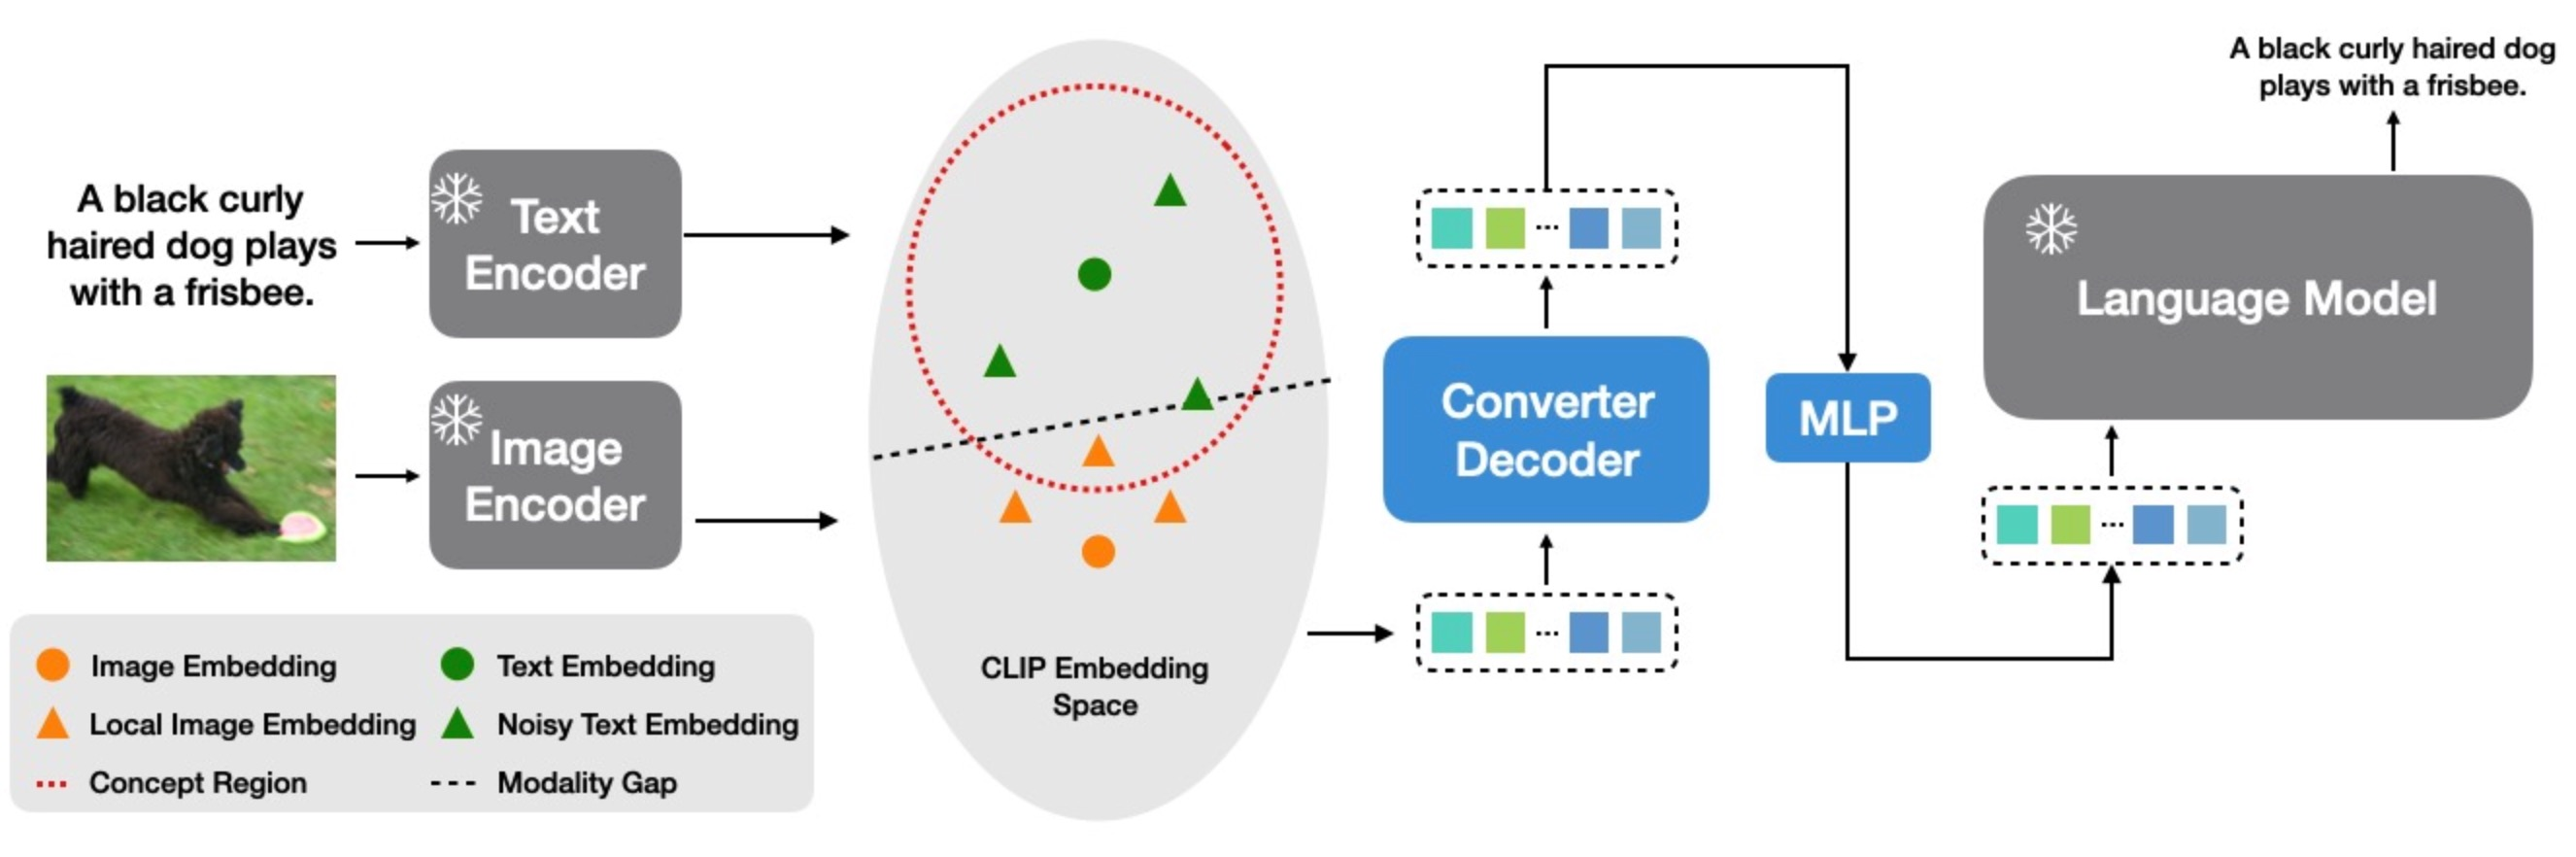
\includegraphics[width=0.98\textwidth]{AnonymousSubmission/LaTeX/asserts/pipeline.png}
%    \caption{\textbf{An overview of MicorCap training and inference pipeline.} First, we encode the input text or image using the CLIP encoders. During training, we inject region noise into the text feature, while we extract an sub-region enhanced image feature during inference. The resulting feature is then fed into the converter decoder to generate a prefix embedding for the language model.}
%     \label{figure:pipeline}
%     \vspace{-0.2cm}
% \end{figure*}

\subsection{Method Overview}
\label{method:definition}
%%%%%%%%%%%%%%%%%%%%%%%%%%%%%%%%%%%%%%%%%%%%%%%%%%%%%%%%%%%%%%%%%%%%%%%%%%%%%%%%%%%%%%%%%%%%%%%%
% 介绍任务定义
%%%%%%%%%%%%%%%%%%%%%%%%%%%%%%%%%%%%%%%%%%%%%%%%%%%%%%%%%%%%%%%%%%%%%%%%%%%%%%%%%%%%%%%%%%%%%%%%%%%
In zero-shot image captioning, the image captioning model is trained with only caption text data. This is possible since CLIP learned a joint space where semantically-related image feature $I_c$ and text feature $T_c$ have closer proximity. By training the model to generate captions conditioned on their CLIP text feature, the model becomes capable of generating captions based on the CLIP image feature without any supervision from paired caption data.

%%%%%%%%%%%%%%%%%%%%%%%%%%%%%%%%%%%%%%%%%%%%%%%%%%%%%%%%%%%%%%%%%%%%%%%%%%%%%%%%%%%%%%%%%%%%%%%%
% 概括任务pipeline,用公式写明CLIP,LLM是freeze住的
%%%%%%%%%%%%%%%%%%%%%%%%%%%%%%%%%%%%%%%%%%%%%%%%%%%%%%%%%%%%%%%%%%%%%%%%%%%%%%%%%%%%%%%%%%%%%%%%%%%
Specifically, we have a caption text corpus $T=\{ t^i | i\in \mathbb{N} \}$ and three network modules, contrastive vision language model CLIP with parameter $\theta_{c}$, pre-trained large language model with parameter $\theta_{l}$ and a learnable adaptor decoder with parameter $\theta$. In text reconstruction training, the adaptor module converts text $t_i$'s CLIP text feature $T_c^{i} \in R^{D}$ to a prefix embedding $E^{i} \in R^{N_q \times D_l}$, where $N_q$ is the length of prefix embedding, $D_l$ is the dimensionality of language model and $D$ is the dimensionality of CLIP feature. The language model generates text $t_i$ based on the prefix embedding $E^{i}$. During training, we freeze the parameter of CLIP $\theta_{c}$ and language model $\theta_{l}$, which makes the adaptor decoder with parameter $\theta$ a plug-and-play module to achieve zero-shot captioning. 
We can formulate the process as follows:
\begin{align}
     \underset{\theta}{\mathrm{maximize}} \quad p(t^i|T_c^{i}, \theta_{c}, \theta_{l})
\end{align}
In inference, CLIP extracts image feature $I_c \in R^{D}$ for an image. The adaptor decoder converts it to prefix embedding and the language model generates a text describing the image content. We present the overall pipeline in Figure~\ref{figure:pipeline} and explain the details of the pipeline in the following sections.

% \subsection{Overall Architecture}
% \label{method:arch}
% Our proposed MacCap consists of three main components: a frozen CLIP, a converter decoder, and a frozen language model, as illustrated in Figure \ref{figure:pipeline}. We briefly introduce the encoding and decoding process of image and/or text in this subsection, followed by detailed training and inference procedure in Section \ref{method:train} and Section \ref{method:inference}.

% \textbf{CLIP Feature Extraction} The frozen CLIP provides image patch feature $I_p \in R^{N_p \times D}$, global feature $I_c \in R^{D}$ and text global feature $T_c \in R^{D}$ where $N_p$ is the image patch number and $D$ is the dimension of CLIP latents space. During text reconstruction training, given a text $T$, a region noise is injected into the text global feature $T_c$ to acquire a text concept region feature $T_{cr} \in R^{N_{cr} \times D}$, where $N_{cr}$ is the length of the converter input sequence. In image-conditioned text generation, given an image $I$, we extract subregion feature augmented image concept region feature $I_{cr} \in R^{N_{cr} \times D}$.

% \textbf{Conditional Text Generation} The converter decoder takes a set of learnable queries and concept region feature as input. Through cross-attention in converter decoder, the learnable queries $Q \in R^{N_q \times D}$ adaptively select informative parts in $T_{cr}$ or $I_{cr}$. The output queries $Q' \in R^{N_q \times D}$ are projected into the language model embedding space by a MLP to acquire a language model prefix embedding $E \in R^{N_q \times D_l}$, where $N_q$ is the number of learnable queries and $D_l$ is the dimension of the language embedding space. Finally, our framework is trained to generate the text based on the prefix embedding $E$.


% \begin{figure*}[t!]
%   \centering
%   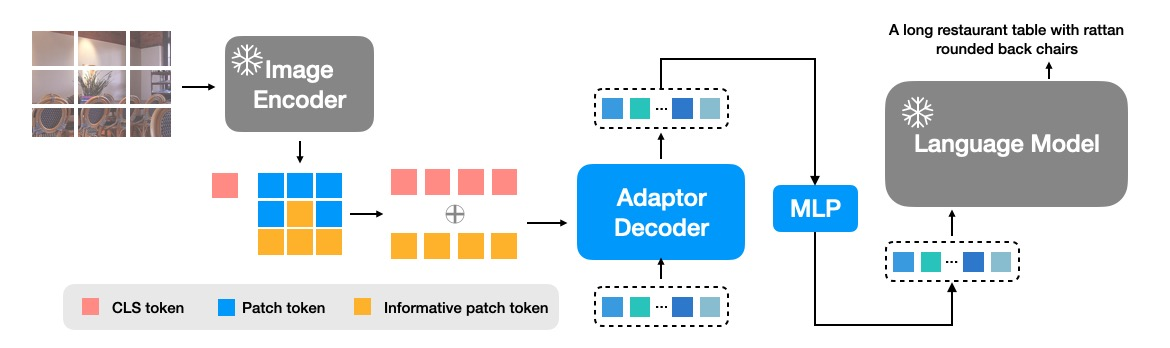
\includegraphics[width=0.98\textwidth]{AnonymousSubmission/LaTeX/asserts/inference_pipeline.jpg}
%    \caption{\textbf{An overview of inference pipeline.} }
%     \label{figure:pipeline}
%     \vspace{-0.2cm}
% \end{figure*}


\subsection{Text Reconstruction Training}
\label{method:train}
%%%%%%%%%%%%%%%%%%%%%%%%%%%%%%%%%%%%%%%%%%%%%%%%%%%%%%%%%%%%%%%%%%%%%%%%%%%%%%%%%%%%%%%%%%%%%%%%
% 1.什么是 Text Reconstruction,
% 2.为什么需要Text Reconstruction(CLIP embedding space)
% 3.为啥需要Region Noise Injected (modality gap)
% 4.Region Noise Injected 利用了analysis里发现的sub matching性质
% 5.设计的motivation(图片由多个caption描述,CLIP space里面点-》text变成多个点表示的distribution-》text)
%%%%%%%%%%%%%%%%%%%%%%%%%%%%%%%%%%%%%%%%%%%%%%%%%%%%%%%%%%%%%%%%%%%%%%%%%%%%%%%%%%%%%%%%%%%%%%%%%%%

\paragraph{\textbf{Region Noise Injection}} The text reconstruction task aims to train our framework to generate text based on the CLIP text features $T_c$, as illustrated in Figure \ref{figure:pipeline}. Our observation on the CLIP Embedding space demonstrates that the gap between the text embedding and subregion image representation satisfies a Gaussian distribution. To mitigate the gap and maintain a consistent format with visual features in inference, we propose region-aware noise injection.
% The motivation is based on the observation that multiple semantically similar captions are required to describe the content in one image due to the mismatch phenomenon. Therefore, we propose to train the model generate text conditioned on a region distribution represented by multiple points in CLIP space, which are multiple CLIP text features $T_c$ injected with different noise in training. Different from previous approaches that learns to generate text from one point in CLIP space, our approach simulates the property in image caption data and acquire more robustness to the \textit{modality gap}.
%%%%%%%%%%%%%%%%%%%%%%%%%%%%%%%%%%%%%%%%%%%%%%%%%%%%%%%%%%%%%%%%%%%%%%%%%%%%%%%%%%%%%%%%%%%%%%%%
% 6.Region Noise Injected 实现细节
%%%%%%%%%%%%%%%%%%%%%%%%%%%%%%%%%%%%%%%%%%%%%%%%%%%%%%%%%%%%%%%%%%%%%%%%%%%%%%%%%%%%%%%%%%%%%%%%%%%
In detail, We first encode $t$ from text corpus $T$ with CLIP text encoder to get text features $T_c$. The $T_c$ is repeated $N_{cr}$ times and added different noise $n_i \in R^{D}, i\in\{1... N_{cr}\}$ from a uniform distribution with zero means and $\sigma$ variance. We apply L2 normalization to the resulting text region feature $T_{cr} \in R^{N_{cr} \times D}$. The process is formulated as follows: 
\begin{align}
    &T_c = \mathrm{CLIP}(t) \in R^{D} \\
    &T_{cr} = \mathrm{Concat}(T_c, T_c, \dots T_c) \in R^{N_{cr} \times D} \\
    &T_{cr}^{i} = \mathrm{L2Norm}(T_{cr}^{i} + n_i) \quad n_i \sim \mathcal{N}(0,\,\sigma^{2})
\end{align}
where $\mathrm{L2Norm}$ is a $l2$-normalization and $\mathrm{Concat}$ is the concatenation operation. The elements in $T_{cr}$ form a cluster of points in the CLIP embedding space centered around $T_c$, which represent captions semantically similar to caption $t$. 

%%%%%%%%%%%%%%%%%%%%%%%%%%%%%%%%%%%%%%%%%%%%%%%%%%%%%%%%%%%%%%%%%%%%%%%%%%%%%%%%%%%%%%%%%%%%%%%%
% 6.Adaptor Decoder 实现细节
%%%%%%%%%%%%%%%%%%%%%%%%%%%%%%%%%%%%%%%%%%%%%%%%%%%%%%%%%%%%%%%%%%%%%%%%%%%%%%%%%%%%%%%%%%%%%%%%%%%
\paragraph{\textbf{Adaptor Decoder}}
The adaptor decoder is designed to project the feature in the CLIP embedding space to the language model embedding space, enabling the language model to generate text based on image or text features in CLIP. Specifically, we have a set of learnable queries $Q \in R^{N_q \times D}$, a transformer decoder \cite{Vaswani2017AttentionIA}, and an MLP module. The learnable queries $Q$ are first updated by self-attention and then fed into a cross-attention module with $T_{cr}$ as the input key and value. The output feature is processed by a feed-forward network to obtain updated learnable queries $Q' \in R^{N_q \times D}$. Finally, $Q'$ is projected by the MLP module to get the prefix embedding $E \in R^{N_q \times D_l}$. The process is formulated as follows:
\begin{align}
    &Q = \mathrm{SelfAttn}(Q) \in R^{N_{q} \times D}  \\
    &Q = \mathrm{CrossAttn}(Q, T_{cr})\in R^{N_{q} \times D} \\
    &Q' = \mathrm{FFN}(Q)\in R^{N_{q} \times D} \\
    &E = \mathrm{MLP}(Q')\in R^{N_{q} \times D_l}
\end{align}
Through cross-attention in the adaptor decoder, the learnable queries $Q$ adaptively select informative parts in $T_{cr}$. At last, the language model generates the input text $t$ based on the prefix embedding $E$. Our objective can be described as:
\begin{align}
   L_{recons}(\theta) = - \frac{1}{|t|} \sum_{i=1}^{|t|} {\log P_{\theta}(w_i|w_{<i}, E, \theta_{c}, \theta_{l}})
\end{align}
where $w_i$ is the $i^{th}$ words in $t$.
% During text reconstruction training, the model is trained to generate text based on a concept regio in CLIP latents. Since semantically coherent image and text embeddings lie within the same concept region, the model is capable of generating image conditioned text.

\subsection{Zero-shot Caption Generation}
%%%%%%%%%%%%%%%%%%%%%%%%%%%%%%%%%%%%%%%%%%%%%%%%%%%%%%%%%%%%%%%%%%%%%%%%%%%%%%%%%%%%%%%%%%%%%%%%
% Inference定义
% inference 最大的challenge利用由analysis得到的subregion信息更贴合caption
%%%%%%%%%%%%%%%%%%%%%%%%%%%%%%%%%%%%%%%%%%%%%%%%%%%%%%%%%%%%%%%%%%%%%%%%%%%%%%%%%%%%%%%%%%%%%%%%%%%
 % Beside, the \textit{modality gap} is alleviated by the region noise injection in text reconstruction training, however, the noise introduce additional uncertainty. We propose multiple sampling and filtering to address the issue.

% Given the fact that MacCap is trained without supervision from paired caption data, the key challenge is to prepare CLIP image feature $I_{cr}$ for caption generation. As observed in CLIP analysi

% reduce the gap between CLIP image feature $I_{cr}$ and text feature $T_{cr}$ fed to adaptor decoder. 

% To address the issue, we propose sub-region feature aggregation and multiple sampling. The pipeline is illustrate in Figure 3.


%%%%%%%%%%%%%%%%%%%%%%%%%%%%%%%%%%%%%%%%%%%%%%%%%%%%%%%%%%%%%%%%%%%%%
% 为什么要sub-region feature aggregation
% sub-region feature aggregation的motivation: CLIP学到的最重要patch不一定是caption需要的patch,所以我们提供更多sub-region信息,有利于caption生成
%%%%%%%%%%%%%%%%%%%%%%%%%%%%%%%%%%%%%%%%%%%%%%%%%%%%%%%%%%%%%%%%%%%%%%
\paragraph{\textbf{Sub-region Feature Aggregation}} 
\label{method:subregion}
Zero-shot caption generation aims to generate captions with a text-only trained adaptor decoder, CLIP, and a language model. Based on our observation that image subregion features exhibit higher similarity to caption features, we propose sub-region feature aggregation to integrate the image global information with subregion information.
% The key challenge is to select informative patch tokens and integrate global image feature $I_c \in R^{D}$ with image patch features $I_p \in R^{N_p \times D}$.
% As we illustrated in CLIP embedding space analysis, the global image feature $I_{c}$ from class token is not always the most important feature to corresponding captions compared with image patch feature $I_p$. The phenomenon demonstrate the image region CLIP focus on is not in line with the image region required for caption generation. To this end, we propose 
%%%%%%%%%%%%%%%%%%%%%%%%%%%%%%%%%%%%%%%%%%%%%%%%%%%%%%%%%%%
% sub-region feature aggregation做法
%%%%%%%%%%%%%%%%%%%%%%%%%%%%%%%%%%%%%%%%%%%%%%%%%%%%%%%%%%%%
Specifically, the ViT-based visual encoder processes images by dividing them into patches and incorporates a class token. In the last layer of ViT, we define the image patch features as $I_{p} \in R^{(N_p + 1) \times D_v}$, where $N_p$ is the number of image patches, $D_v$ is the dimensionality of ViT and the first element in $I_{p}$ is the class token $I_{p}[0]  \in R^{D}$. 
% Each element in $I_{p}$ contain an attention weight $A^i \in R^{N_p \times N_p}, i \in \{0, 1 \dots N_p \}$. 
The global image feature $I_{c} \in R^{D}$ is obtained by a linear projection on class token $I_{p}[0]$. We select the patches with the top $N_{cr}$ score in the class token's attention weight and denote them as informative patch tokens. The subregion features $I_{s} \in R^{N_{cr} \times D} $ are obtained by aggregating patch features in informative patch based on corresponding attention weight $A \in R^{N_{cr} \times (N_p + 1)}$. Finally, the subregion-enhanced image feature $I_{cr} \in R^{N_{cr} \times D}$ is acquired by taking the average of $I_{c}$ and $I_{s}$. The process can be formulated as follows:
\begin{align}
    &I_{p}' = \mathrm{Linear}(I_{p}) \in R^{(N_p + 1) \times D}  \\
    &I_{c} =  I_{p}'[0] \in R^{D} \\
    &I_{s} = A  I_{p}' \in R^{N_{cr} \times D} \\
    &I_{cr} = \mathrm{Concat}(I_{s}^1 + I_{c}, \dots, I_{s}^{N_{cr}} + I_{c})  \in R^{N_{q} \times D}
\end{align}
where $I_{p}'$ is the projected image patch features, and $\mathrm{Linear}$ is the linear projection that projects visual features to CLIP multimodal embedding space. The $I_{cr}$ represents the image feature in CLIP space and is used to generate text in the same way as text region feature $T_{cr}$. 


% the image class token feature is a weighted sum of patch features $I_{p}$ decided by the attention weight $A_c \in R^{N_p \times N_p}$. We denote the patch features with top $N_{cr}$ score in $A_c$ as informative subregions. The subregion features $I_{tp} \in R^{N_p \times D}$ are obtained by taking the weighted sum of patch features $I_{p}$ based on the weights from corresponding attention weight $A_p^{i} \in R^{N_p \times N_p}, i \in \{0, 1 \dots N_p - 1 \}$. Finally, the CLIP subregion enhanced image feature $I_{cr}$ is acquired by the sum average of  $I_{c}$ and $I_{tp}$. We can formulate the process as following:
% \begin{align}
%     &I_{c} = \mathrm{Proj}(I_{p} @ A_c.T) \in R^{D}  \\
%     &Q = \mathrm{CrossAttn}(Q, T_{cr})\in R^{N_{q} \times D} \\
%     &Q' = \mathrm{FFN}(Q)\in R^{N_{q} \times D} \\
%     &E = \mathrm{MLP}(Q')\in R^{N_{q} \times D_l}
% \end{align}


\begin{figure}[t!]
  \centering
  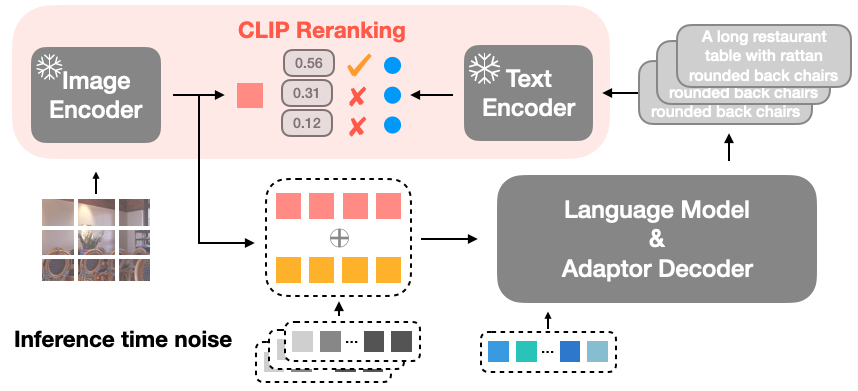
\includegraphics[width=0.45\textwidth]{AnonymousSubmission/LaTeX/asserts/rerank.png}
   \caption{\textbf{Multiple sampling and filtering pipeline} During inference, each image uses noise to generate several different captions, which are reranked by CLIP to output the best.}
    \label{figure:rerank}
\end{figure}


\paragraph{\textbf{Multiple Sampling and Filtering}} 
%%%%%%%%%%%%%%%%%%%%%%%%%%%%%%%%%%%%%%%%%%%%%%%%%%%%%%%%%%%
% Multiple Sampling and Filtering motivation (noise定义相关)
% Multiple Sampling and Filtering 具体做法
%%%%%%%%%%%%%%%%%%%%%%%%%%%%%%%%%%%%%%%%%%%%%%%%%%%%%%%%%%%%
The \textit{modality gap} is alleviated by the region noise injection in text reconstruction training, however, the noise introduces additional uncertainty. We propose a \textit{multiple sampling and filtering} strategy that incorporates inference-time noise and CLIP reranking to address the issue and boost performance, which is illustrated in Figure~\ref{figure:rerank}. Specifically, we introduce inference time noise sampled from a normal distribution $\mathcal{N}(0,\sigma^{2})$ into the subregion enhanced image feature $I_{cr} \in R^{N_{cr} \times D}$. We generate text based on the perturbed subregion enhanced image feature $I_{cr}$, and repeat this process $S$ times to generate $S$ diverse texts. CLIP is utilized to evaluate the cosine similarity between the generated texts and the image. We select the text with the highest similarity as the predicted image caption. This strategy leverages CLIP knowledge to improve the generation quality of our model.

% \label{method:inference}
% % motivation有两个,第一个是analysis部分发现的subregion 信息会跟贴和text embedding,所以使用一种聚合子区域图片信息的算法来增强image feature,第二个motivation是根据concept region的定义,在这个区域内的信息都是有语义信息的,所以我们采取一种在concept region内加noise多次sample加筛选的方法来mining the region
% Image conditioned text generation aims to generate texts related to the semantic content in the visual input. As \ref{analysis:subregion} demonstrate that image subregion features contains valuable semantic information which can be utilized to navigate the image global feature $I_{c}$. We propose to aggregate sub-region features from image patch feature $I_p$ to acquire a comprehensive image concept region feature $I_{cr}$. Specifically, we provide an outline of the algorithm in Algorithm \ref{algo:inference}.

% \begin{algorithm}[t] 
% 	\caption{Image Subregion Features Aggregation} 
%     \renewcommand{\algorithmicrequire}{\textbf{Input:}}
%     \renewcommand{\algorithmicensure}{\textbf{Tips:}}
% 	\label{algo:inference} 
% 	\begin{algorithmic}[1]
% 		\REQUIRE $M$: CLIP visual encoder;$Proj$: CLIP visual projector;$I$: image input;
%         \ENSURE $A \in R^{N_p \times N_p}$ is the attention map from last layer of CLIP visual encoder.
% 		\STATE $I_p, A \gets Proj(M(I)) $ \textcolor{gray}{\# Embed image and get attention map}
% 		\STATE $I_c \gets I_p[0]$ \textcolor{gray}{\# Image global feature}
% 		\STATE $Idx \gets Topk(A[0, :], N_{cr})$ \textcolor{gray}{\# Select $N_{cr}$ patches response most to image global feature}
%         \STATE $I_{cr} \gets []$ \textcolor{gray}{\# Init a empty list}
% 		\FOR{$i$ in $Idx$} 
%             \item \textcolor{gray}{\# Aggregate visual feature on each selected patch}
%             \item $L \gets A[i, :] \cdot I_p + I_c$ \textcolor{gray}{\# Aggregation other patches based on attention score}
%             \item $I_{cr}[i] \gets \mathrm{L2Norm}(L)$ \textcolor{gray}{\# Append patch feature to the list after l2 normalization}
%         \ENDFOR
%         \STATE $I_{cr} \gets concat(F)$ \textcolor{gray}{\# Concat patch-level features to get image concept region feature}
% 	\end{algorithmic} 

% \end{algorithm}

% In Algorithm \ref{algo:inference}, we describe a method for extracting the image concept region feature $I_{cr}$. This is achieved by aggregating visual features from sub-regions of an image, selected based on their response scores to the image class token in the CLIP visual encoder. The obtained scores suggest that the features extracted from these regions encompass abundant semantic information while also maintaining diversity compared to the global image feature, $I_c$.
% The resulting image concept region feature, $I_{cr}$, represents a concept region of visual semantic content in CLIP latents that is consistent with the training objective.
% The converter decoder dynamically combines a sequence of subregion-refined image features using learnable queries $Q$ to obtain the aggregated query $Q'$. The prefix embedding $E$ is extracted by projecting $Q'$ to language model embedding space. The generation process can be described as:
% \begin{align}
%    \hat{w_i}(\theta) = \mathop{\arg\max}_{ w_i \in V} P_{\theta}(w_i|\hat{w}_{<i}, E)
% \end{align}
% where $\hat{w_i}$ is the $i^{th}$ predicted word and V is the vocabulary.

% \subsection{Multiple Sampling and Filtering}
% \label{method:sample}
% The \textit{concept region} is composed of image/text embeddings with similar semantic information. Based on this, we propose a \textit{multiple sampling and filtering} strategy that incorporates inference-time noise and CLIP reranking to mining the concept region. 
% % Specifically, we inject $k$ different inference time noise $\mathcal{N}(0,\,\sigma_i^{2})$ into the image concept region feature $I_{cr}$ resulting in $K$ different image concept region features $I_{cr}$. The converter decoder extracts the corresponding $Q_i, i \in {1,2,\dots,K}$ from these $K$ concept region features $I_{cr}$. After projection, we obtain $k$ prefix embeddings $E_i, i \in {1,2,\dots,K}$, which are concatenated to form the final prefix embeddings $E \in R^{K \times D_l}$. 
% Specifically, we introduce $N_{cr}$ inference time noise samples from a normal distribution $\mathcal{N}(0,,\sigma^{2})$ into the image concept region feature $I_{cr} \in R^{N_{cr} \times D}$.
% We generate text based on the perturbed image concept region feature $I_{cr}$, and repeat this process $S$ times to generate $S$ diverse texts. 
% The CLIP is utilized to evaluate the cosine similarity between the generated texts and the image. We select the text with the highest similarity as the predicted image caption. This strategy helps to exploit the concept region, resulting in more accurate text generation.

% \paragraph{\textbf{Zero-shot Visual Question Answering with Captioning}}
\subsection{Zero-shot Visual Question Answering with Captioning}
In this part, we illustrate the potential extensibility by showing the pipeline for zero-shot VQA with text-only trained MacCap. As there is no supervision from VQA data, we convert the image into a caption by MacCap. To answer the question about the image, we only use the LLM in MacCap to do open-end text generation based on a VQA prompt. The prompt contains the question and image caption, which is \textit{"[caption] Question: [question] Answer:"}. Given the inherent difficulty of the zero-shot VQA task, we transform the VQA task into an image-text retrieval task. Specifically, the generated answer is embedded by the CLIP text encoder and computed cosine similarity with CLIP text embedding from answer candidates.